\chapter{Measuring compiler framework performance}
\label{chap:measuring-compiler-performance}

%% Introduction
% Hook
In this chapter, we measure the runtime performance of two user-extensible compiler frameworks: MLIR and xDSL.
% Argument
The usefulness of these measurements are three-fold. First, we provide insight into the performance of the current versions MLIR and xDSL in relation to each other. % interesting in its own right, and as a baseline for optimisation
Second, we identify the components of xDSL's implementation which contribute most to its overall runtime, and as such are the best targets for optimisation (\autoref{chap:specialising-optimising-pattern-rewriting}) as a corrollary of Amdahl's law \cite{amdahlValiditySingleProcessor1967}.
Finally, we isolate small, self-contained components of the implementation which are comparable between MLIR and xDSL, through which the impact of dynamism can be examined (\autoref{chap:dynamism-pattern-rewriting}).
% Link



\section{Methodology}
\label{sec:methodology}

%% Short intro
% Hook
Accurate performance measurement is a fundamental yet notoriously fickle discipline in systems research.
% Argument
In this section, we discuss our experimental methodology, including: the hardware and software setup; the selection of workloads examined; and additional infrastructure constructed.
% Link
Through this, we aim to justify our experimental procedure and facilitate reproducibilty of results.

\subsection{Experimental setup}
\label{ssec:experimental-setup}

% Hook
All experimental results for this work were measured with the same experimental setup: an AWS EC2 virtual machine (\autoref{tab:experimental-setup}).
% Argument
This choice benefits experimental replicability, making it easy for future researchers to provision their own AWS EC2 instance with a similar machine configuration, and hence performance characteristics.
However, there are also drawbacks associated with using virtualised cloud infrastructure for performance measurements.
Unlike bare-metal machines, the added layer of indirection of the hypervisor adds noise and confounding effects to the performance measurements.
We use the subset of machine configuration available through the hypervisor to minimise noise, for example by pinning workloads to invididual virtual cores and disabling address space randomisation. % Things done by pyperf
Following these mitigations, the experimental setup is a fair compromise of leveraging available resources and empowering reproducibility for slightly reduced experimental precision.
Finally, the ubiqitous use of cloud resources, especially for compilation workloads in build servers, makes this choice and its associated properties representative of real-world applications.
% Link

\begin{table}[H]
  \caption{Summary of the experimental setup used for performance measurement.}
  \label{tab:experimental-setup}
  \centering
  \begin{tabular}{lll}
    \toprule
    \textbf{Configurable} & \textbf{Configuration} \\
    \midrule
    AWS instance type & c5a.4xlarge EC2 \\
    Operating system & Debian 24.04 (Noble) \\
    Linux kernel version &  \\
    \midrule
    CPU name & AMD EPYC 7R32 \\
    Logical CPU cores & $16$ \\
    Clock frequency [MHz] & $2799.99$ \\
    L1 Data Cache [KiB] & $32$ \\
    L1 Instruction Cache [KiB] & $32$ \\
    L2 Unified Cache [KiB] & $512$ \\
    L3 Unified Cache [KiB] & $16384$ \\
    RAM [GB] & 16 \\
    \bottomrule
  \end{tabular}
\end{table}

% Hook
In addition to the underlying experimental hardware, the software configuration of the machine significantly contributes to its performance characteristics.
% Argument
As such, we similarly provide a description of the language versions and build tools, along with the exact \texttt{git} SHAs of the compilation frameworks being compared in this chapter (\autoref{tab:experimental-configuration}).
% Link
Experiments in later chapters ablate across both language and framework versions, with these versions being noted explicitly when changed.

\begin{table}[H]
  \caption{Summary of experimental software configuration used for performance measurement.}
  \label{tab:experimental-configuration}
  \centering
  \begin{tabular}{lll}
    \toprule
    \textbf{Configurable} & \textbf{Configuration} \\
    \midrule
    CMake version & 3.28.3 \\
    Ninja version & 1.11.1 \\
    \midrule
    Python interpreter & CPython 3.10.17 \\
    C++ compiler & clang 18.1.8 \\
    \midrule
    xDSL commit SHA & \texttt{3fcc65b5} \\
    MLIR commit SHA & \texttt{6516ae4} \\
    \bottomrule
  \end{tabular}
\end{table}


\subsection{Experimental workloads}
\label{ssec:experimental-workloads}

%% Use the same textual IR since xDSL is a sidekick compiler
% Hook
One novel contribution of xDSL is the concept of sidekick compilation frameworks: ``an approach that uses multiple frameworks that interoperate with each other by leveraging textual interchange formats [...]'' \cite{fehrXDSLSidekickCompilation2025}.
% Argument
We leverage xDSL's interoperability with \ac{mlir}'s textual \ac{ir} to construct workloads which can be applied to both frameworks.
This guarantess directly comparable performance measurements at the pipeline phase and function level, driven by the shared representation.
Without sidekick compilation, for example comparing two more disparate user-extensible compiler frameworks such as MLIR and Pliron \cite{vaivaswathanagarajVaivaswathaPliron2025}, this comparison would be constrained to only end-to-end measurement, obscuring the impact of variables such as dynamism on the performance properties.
% Link

%% Want to pick things which are simple enough to examine in detail but complex enough to exercise interesting properties of the machine.
% Hook
\ac{mlir}'s textual \ac{ir} is incredibly expressive, facilitating representation of algorithms of varying complexity across a wide range of abstraction levels.
% Argument
In this case, we consider workloads to be the combination of a rewriting optimisation and a segment of \ac{ir} which optimises it. This can be used to drive both the two frameworks' command line optimiser tools and internal phases and functions within the frameworks.
% Simple enough to reason deeply about, but exercises common pattern rewriting dependencies like replacing ops, checking traits, ... (all quite dynamic)
To maximise the signal measured by our experiments, we prefer workloads which are sufficiently simple examine is significant detail, but also exercise a wide variety of the functionality supported by % and common idioms of
pattern rewriting machinery.
Furthermore, whilst making experimental data representative of real-world workloads is an admirable goal, it is orthogonal to our exploration of the impact of dynamism on user-extensible compiler infrastructure.
Constructing truly representative workloads is a significant task in itself, requiring the survey of all common use cases of compiler infrastructure and thus out of scope of this thesis.
% Link
As such, we predominantly focus on simple but non-trivial optimisations such as constant folding.

\subsubsection{Constant folding}
\label{sssec:experimental-workload-constant-folding}

% Hook
Stoltz et al. define constant folding as ``a well-known static compiler technique in which values of variables which are determined to be constants can be passed to expressions which use these constants'' \cite{stoltzConstantPropagationFresh1994}.
% Argument
It has been leveraged for both performance and space improvements since the earliest optimising compilers. Despite this, it remains relevant even over more modern, exotic optimisations due to its simplicity, efficient implementation, and high impact on generated \ac{ir}.
In addition to this, procedural generation of the workload \ac{ir} can be simply parameterised in length (\autoref{sec:constant-folding-workload-impl}), facilitating experiments examining performance scaling.
% Link
An example \ac{ir} segment with three constants is shown below (\autoref{listing:constant-folding-workload-example}).

% \vspace{2em}

\begin{figure}[H]
    \centering
    \begin{subfigure}[b]{0.45\textwidth}
       \centering
        \begin{minted}[fontsize=\footnotesize]{text}
            builtin.module {
              %0 = arith.constant 865 : i32
              %1 = arith.constant 395 : i32
              %2 = arith.addi %1, %0 : i32
              %3 = arith.constant 777 : i32
              %4 = arith.addi %3, %2 : i32
              "test.op"(%4) : (i32) -> ()
            }
        \end{minted}
        \label{listing:constant-folding-workload-initial}
        \caption{Unfolded \ac{ir} amenable to constant folding.}
    \end{subfigure}
    \hfill
    \begin{subfigure}[b]{0.45\textwidth}
        \centering
        \begin{minted}[breakanywhere,fontsize=\footnotesize]{text}
            builtin.module {
              %0 = arith.constant 2037 : i32
              "test.op"(%0) : (i32) -> ()
            }
        \end{minted}
        \footnotesize\vspace{2.5em}
        \caption{Constant folded \ac{ir}.}
        \label{listing:constant-folding-workload-folded}
    \end{subfigure}
    \vspace{1em}
    \captionsetup{name=Listing}
    \caption{Folding three integer constants over arithmetic addition in \ac{mlir}'s textual \ac{ir}.}
    \label{listing:constant-folding-workload-example}
\end{figure}

\vspace{2em}


\subsection{Measurement infrastructure}
\label{ssec:infrastructure}

%% Warmed timeit and stuff
% Hook
In order to facilitate the efficient and reproducible measurement of xDSL's performance characteristics, we developed infrastructure to drive our benchmarks with a variety of measurement tools and profilers.
% Argument
% Link
%% Corrollary benefits
% Hook
In addition to their usefulness for understanding and optimising compiler performance, the benchmarks composing the performance experiments also provide an opportunity to augment the development process of the xDSL project.
% Argument
Benchmarks can be used to characterise the performance impact of changes to the xDSL codebase, making it easier to avoid unnecessary performance regression.
As such, we provide a command line interface for developers to run the benchmarks, with further functionality which supports a variety of profiling tools. % TODO: Does this get moved up a paragraph?
Furthermore, our benchmarks are constructed to interface with Airspeed Velocity \cite{michaeldroettboomAirspeedvelocityAsv2025}, a tool which runs benchmarks across repository commits. This information is tracked on the xDSL website \url{https://xdsl.dev/xdsl-bench/}, providing a dashboard for the performance characteristics of xDSL over time.
% Link


















\section{End-to-end benchmarks}
\label{sec:e2e-benchmarks}

%% Introduction, goals
% Hook
The simplest metric for the performance of a system is its overall runtime.
% Argument
As such, a good place to start comparing the performance characteristics of MLIR and xDSL is the end-to-end performance of their command line tools.
% Link
Whilst end-to-end measurements are well-aligned metrics of performance for real-world workloads, they are limited by their coarse granularity. Conveniently, modern compiler frameworks are structured in a way that facilitates more detailed metrics even for end-to-end runs. % TODO: Does this duplicate the earlier workload stuff?
One of LLVM's key insights was that compilation can be split into a sequence of discrete steps, avoiding the complex interleaved control logic of previous state-of-the-art compilers.
% Argument
As such, compilers having LLVM's pedigree, such as MLIR and xDSL, can be modelled as a pipeline -- parsing the input, applying optimisation transformations, and generating a lowered output.
This allows us to break down end-to-end benchmarks into components of finer granularity for free.
% Link

%% Methodology
% Hook
% Argument
For MLIR, we invoke \texttt{mlir-opt constant\_folding.mlir --canonicalize --mlir-timing}. By default, this prints results to four decimal places, which is insufficiently granular to time printing very short \ac{ir} segments. As such, we modify MLIR's implementation to print more decimal places. In order to guarantee statistical significance following this change, we measure across ten repeats. Since we are sampling a single variable, we take the arithmetic mean of these values, with an uncertainty given by their standard deviation.
For xDSL, we leverage our custom benchmarking infrastructure (\autoref{ssec:infrastructure}), which drives each phase canonicalsing the workload and records precise timings. We then calculate the average and uncertainty by the same procedure.
% Link
These wall times for each framework and the slowdown between them can then be plotted (\autoref{fig:end-to-end-constant-folding-walltime}).

% Figure: relative performance bar chart
%% Constant folding example. Short but complex example with lots of rewrites?
\begin{figure}[H]
    \centering
    \begin{subfigure}[b]{0.45\textwidth}
        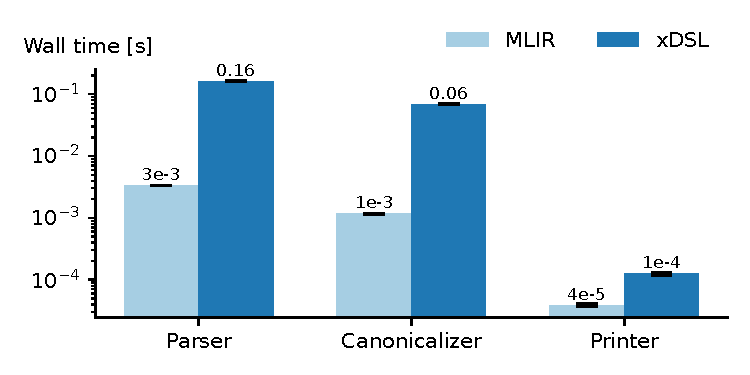
\includegraphics[width=\textwidth]{images/measuring_compiler_performance/walltimes.pdf}
        \vspace{0.5em}
        \caption{All pipeline phases of MLIR are faster than xDSL.}
        \vspace{0.5em}
        \label{fig:end-to-end-constant-folding-walltime}
    \end{subfigure}
    \hfill
    \begin{subfigure}[b]{0.45\textwidth}
        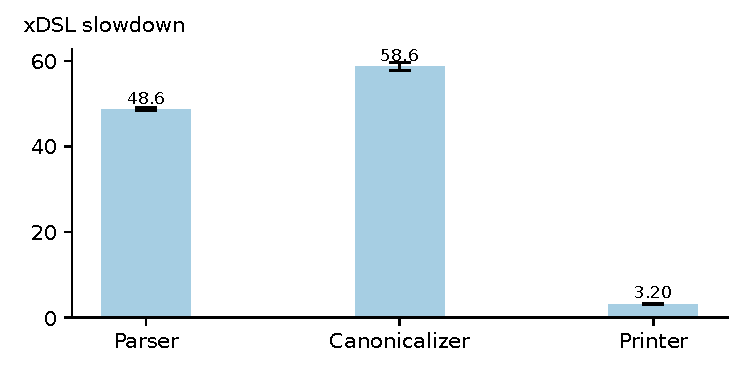
\includegraphics[width=\textwidth]{images/measuring_compiler_performance/speedup.pdf}
        \caption{xDSL's parser and canonicalizer incur around $50\times$ slowdown, whereas the printer slows down only $2\times$ for small workloads.}
        \label{fig:end-to-end-constant-folding-speedup}
    \end{subfigure}
    \caption{Performance comparison of constant folding $1000$ integer addition operations (\autoref{sssec:experimental-workload-constant-folding}) between xDSL and MLIR.}
    \label{fig:end-to-end-constant-folding}
\end{figure}


%% Discuss results
% Hook
Despite its simplicity, this initial experiment reveals a number of interesting insights.
% Argument
Firstly, the slow-down from xDSL to MLIR for the first two passes is approximately $50\times$. This provides an initial baseline for the overhead incurred by the combination of xDSL's language runtime and implementation details over the MLIR implementation.
Secondly, the slow-down for the printer is much lower that the other two phases, at only $3\times$. % TODO: Pull in uploaded graphs
This is because the constant folded output is very short, containing only two \ac{ir} instructions (\autoref{listing:constant-folding-workload-folded}) for any length input of that schema. As such, the overhead of writing to the standard output is greater than the processing time for those few operations. In contrast, the logic implement parsing and canonicalisation rewrites is much longer than any fixed overhead they incur, such as the parser reading the \ac{ir} from a file.
% Link

% Hook
Since the parser represents a majority of the total runtime for both frameworks, it appears an attractive candidate for optimisation as a corrollary of Amdahl's law. This is because improving it by a fixed proportion would result in the greatest runtime reduction than any other pipeline phase.
% Argument
Despite this, we select the pattern rewriting phase, which implements the canonicalizer, for further investigation.
This is because the complexity of modern compilers is almost exclusively focussed on rewrites for optimisation, with both parsing and printing being broadly solved problems. In addition to this, the parser and printer are used only for debugging in many use cases, with the compiler framework predominantly being used for its rewriting capabilities. Examples of this include XLA \cite{sabne2020xla} emitting \ac{mlir} \ac{ir} in custom dialects, using \ac{mlir}'s rewrite machinery to lower code to the target hardware.
Furthermore, the rewriter is a much more dynamic workload, with its control flow necessarily determined at runtime based on the contents of the \ac{ir} being optimised.
% Link
This further makes it a more suitable candidate for examination through the lens of the impact of dynamism on user-extensible compiler frameworks.
% Secondly, it has the smallest slowdown of the pipeline phases (\autoref{fig:end-to-end-constant-folding-speedup}), suggesting other phases may have more opportunities for optimisation before being bounded by properties of the language runtime.








% TODO: Do we even need this section? What does it add -- nothing since repeats less well what we do in specialisation. Just need to segue effectively to micro-benchmarks

% \section{Pattern rewriting}
% \label{sec:pattern-rewriting}

% %% Introduction
% % Hook
% Having selected pattern rewriting as the compilation phase to examine in detail, we can modify our benchmarks to drive only
% % Figure: MLIR vs xDSL scaling across workloads?
% % Figure: Trace of MLIR and xDSL overall?












\section{Micro-benchmarks}
\label{sec:ubenchmark}

% Hook
Micro-benchmarking refers measuring the performance of fast, granular, and isolated segments of code.
% Argument
The term was coined by Saavedra et al. in their 1995 paper \cite{saavedraPerformanceCharacterizationOptimizing1995} ``Performance Characterization of Optimizing Compilers''. As such, we are in good company in our application of micro-benchmarking approaches to this problem domain.
Micro-benchmarks have many desirable properties. Since they run quickly, they can cheaply be repeated for statistical confidence.
Furthermore, their fine granularity makes them tractable to reason about -- providing useful information to optimise the component of the system they measure.
However, a key difficulty of micro-benchmarking is ensuring alignment with overall system performance. For example, the selection of code paths to micro-benchmark may introduce bias, making them less representative of the overall system. In addition to this, their performance may be inflated as a consequence of warmed caches and JIT optimisations across repeats, which would not occur during normal operation.
% Link
As such, micro-benchmarking is a useful tool for deeply understanding the performance of software, but must be used carefully to ensure the validity of its results.

% Hook
As discussed in our related work (Section \ref{sec:perf-user-extensible-frameworks}), Amini and Nui's talk ``How Slow is MLIR'' \cite{aminiHowSlowMLIR2024} discusses a set of micro-benchmarks for key operations in the MLIR compiler, such as traversing the IR and creating operations.
% Argument
These micro-benchmarks were used to inform the optimisation of MLIR's data structures and for comparison with traditional LLVM-based compilers. The implementation of the micro-benchmarks allude to an underlying design goal in MLIR by their measurement of asymptotic scaling properties\footnote{\url{https://github.com/joker-eph/llvm-project/blob/6773f827b9ee8055063fcf6b2c6fcdc7f4f579d2/mlir/unittests/Benchmarks/Cloning.cpp\#L66}}. This design goal is asymptotically optimal performance for its underlying data structures. However, data structures with these characteristics often incur constant-time penalties.
This causes overhead for small workloads, where, unlike the asymptotic case, the cost is not amortised. As such, micro-benchmarks may not be representative of the system's overall performance, revealing possibility for the optimisation of code co-designed using them.
Despite this, they can still provide useful insight into MLIR's performance characteristics.
% Link
We implement micro-benchmark workloads for the xDSL equivalent to those for MLIR presented in the keynote, and compare the results of these benchmarks between the two implementations, giving insights into their relative performance.
% We further leverage profiling tools to examine the execution of the two implementations. This allows us to distinguish the cost incurred by the language runtime from the cost incurred by the algorithmic approach of the implementation.

\subsection{Implementation}
\label{ssec:ubenchmark-implementation}

%% Finding and building the MLIR microbenchmarks
% Hook
Unfortunately, the implementation and build instructions for the ``How Slow is MLIR?'' micro-benchmarks were not published with the talk.
% Argument (too informal?)
However, their source code can be found on a branch of the presenter's fork of LLVM\footnote{\url{https://github.com/joker-eph/llvm-project/tree/benchmarks}}. We provide a copy of this source code and instructions for running the benchmarks\footnote{\url{https://github.com/EdmundGoodman/llvm-project-benchmarks}} to enhance the replicability of our results and facilitate further performance experiments.
% Link
This source code can then be used to construct comparable micro-benchmarks in Python.

%% Design of our microbenchmarks
% Hook
A key design goal of our micro-benchmarks for xDSL is parity with those provided for MLIR, ensuring the validity their direct comparison.
% Argument
As such, their implementation was derived from the MLIR benchmarks, matching test data and function invocations as closely as possible.
In addition to being fairly comparable, it is critical that the micro-benchmark results are statistical significant. This is particularly challenging as their execution time approaches the $1$ns resolution of the most granular system counters on the benchmarking machine. As such, we measure the total time taken to execute the functions under test $32768$ times, evaluating the individual duration by dividing by the number of iterations. As with the traditional benchmarks, this process is repeated ten times, calculating the arithmetic mean and standard deviation as the value and its uncertainty respectively.
% Link
In the following sections, we discuss the implementations of a number of micro-benchmarks, facilitating discussion of the insights they give into compiler performance across implementations and language runtimes in later chapters.


\subsection{Operation instantiation}
\label{ssec:ubenchmark-operation-instantiation}

% Hook
Operations are a central data structure in MLIR and xDSL's \ac{ir} representation, constituting dialects and composing together into programs.
% Argument
As such, the methods to instantiate operations a very frequently invoked, making them a good candidate for micro-benchmarking.
% Link
In both MLIR and xDSL, there are two main ways an operation can be constructed: direct creation \circledbase{pairedOneLightBlue}{1}; or using an builder \circledbase{pairedTwoDarkBlue}{2} (Listing \ref{listing:ubenchmark-op-creation-bench}).

\begin{figure}[H]
    \centering
    \begin{subfigure}[b]{0.45\textwidth}
       \centering
        \begin{minted}[fontsize=\footnotesize,escapeinside=$$]{text}
            // Setup
            OpBuilder b(ctx.get());

            // Benchmarks
            OperationState opState(unknownLoc, "testbench.empty"); $\circledbase{pairedOneLightBlue}{1}$
            Operation::create(opState);
            b.create<EmptyOp>(unknownLoc); $\circledbase{pairedTwoDarkBlue}{2}$
        \end{minted}
        \caption{``How Slow is MLIR?'' C++ implementation.}
        \label{listing:ubenchmark-op-creation-bench-mlir}
    \end{subfigure}
    \hfill
    \begin{subfigure}[b]{0.45\textwidth}
        \centering
        \begin{minted}[fontsize=\footnotesize,escapeinside=$$]{text}
            # Setup
            EMPTY_OP = EmptyOp()

            # Benchmarks
            EmptyOp.create() $\circledbase{pairedOneLightBlue}{1}$
            EmptyOp.build()  $\circledbase{pairedTwoDarkBlue}{2}$
        \end{minted}
        \footnotesize\vspace{2em}
        \caption{xDSL Python implementation.}
        \label{listing:ubenchmark-op-creation-bench-xdsl}
    \end{subfigure}
    \vspace{1em}
    \captionsetup{name=Listing}
    \caption{Micro-benchmark implementations for methods checking an operation has a trait.}
    \label{listing:ubenchmark-op-creation-bench}
\end{figure}

% Hook
The performance characteristics of these implementations differ significantly (\autoref{tab:ubenchmark-op-creation}).
% Argument
In MLIR, the creation and building mechanisms have approximately the same performance, taking around $150$ns to instantiate an operation. In contrast, xDSL's operation building is much slower than direct creation, jumping from $20\times$ to $80\times$ slower. This comes as a result of the trade-off xDSL makes between performance and expressivity, with its builder including a large section of inference and verification logic as a wrapper around the create method.
% Link


\begin{table}[H]
  \caption{Operation instantiation in xDSL is approximately $20\times$ slower than in MLIR when creating instructions in the asymptotic case, but is up to $80\times$ slower when using the builder API.} %, repeated ten times over $32768$ operations. Methodology is discussed in detail in Appendix \ref{} to facilitate replicability.}
  \label{tab:ubenchmark-op-creation}
  \centering
  \begin{tabular}{lcc}
    \toprule
    \textbf{Mechanism} & \textbf{MLIR [ns]} & \textbf{xDSL [ns]}\\
    \midrule
    $\circledbase{pairedOneLightBlue}{1}$ Create & $155 \pm 14$ & $3600 \pm 1500$ \\
    $\circledbase{pairedTwoDarkBlue}{2}$ Build & $153 \pm 0.5$ & $12100 \pm 1900$ \\
    \bottomrule
  \end{tabular}
\end{table}




\subsection{Operation trait checks}
\label{ssec:ubenchmark-trait-checks}

%% Micro-benchmark motivation and details
% Hook
Traits are a key property of MLIR and xDSL's operations, providing a mechanism to abstract implementation details and properties.
% Argument
In order to allow users of the frameworks to leverage an operation's trait information, both MLIR and xDSL provide helper methods to check whether an operation has a certain trait.
These methods are used very frequently in common tasks. For example, when pattern rewriting over a block of IR, the traits of the block's constituent operations are often used by the matching engine to identify valid rewrites.
% Link

\begin{figure}[H]
    \centering
    \begin{subfigure}[b]{0.45\textwidth}
       \centering
        \begin{minted}[fontsize=\footnotesize]{text}
            // Setup
            Operation op = b.create<OpWithRegion>(
                unknownLoc
            );

            // Benchmark
            bool hasTrait = op->hasTrait<
                OpTrait::SingleBlock
            >();
        \end{minted}
        \caption{``How Slow is MLIR?'' C++ implementation.}
        \label{listing:ubenchmark-trait-checks-bench-mlir}
    \end{subfigure}
    \hfill
    \begin{subfigure}[b]{0.45\textwidth}
        \centering
        \begin{minted}[fontsize=\footnotesize]{text}
            # Setup
            op = OpWithRegion()

            # Benchmark
            has_trait = op.has_trait(SingleBlock)
        \end{minted}
        \footnotesize\vspace{2em}
        \caption{xDSL Python implementation.}
        \label{listing:ubenchmark-trait-checks-bench-xdsl}
    \end{subfigure}
    \vspace{1em}
    \captionsetup{name=Listing}
    \caption{Micro-benchmark implementations for methods checking an operation has a trait.}
    \label{listing:ubenchmark-trait-checks-bench}
\end{figure}

% Hook
These methods can be simply benchmarked for an example workload (Listing \ref{listing:ubenchmark-trait-checks-bench}).
% Argument
However, care must be taken when implementing these benchmarks to ensure they are can be equitably compared. For example, the operations must both have the same number of traits, and the trait being checked must be at the same position in that operation's list of traits.
If this is not true, one implementation may require fewer iterations to perform its workload, invalidating the comparability of the two results.
% Link
Micro-benchmarks of checking traits for both implementations show a slow-down of approximately $240\times$ from MLIR to xDSL (\autoref{tab:ubenchmark-trait-checks}).

\begin{table}[H]
  \caption{Trait checks in xDSL are approximately $240\times$ slower than in MLIR in the asymptotic case.} %, repeated ten times over $32768$ operations. Methodology is discussed in detail in Appendix \ref{} to facilitate replicability.}
  \label{tab:ubenchmark-trait-checks}
  \centering
  \begin{tabular}{cc}
    \toprule
    \textbf{MLIR [ns]} & \textbf{xDSL [ns]}\\
    \midrule
    $3.89 \pm 0.01$ & $924 \pm 513$ \\
    \bottomrule
  \end{tabular}
\end{table}


% % Hook
% The trait checking micro-benchmark yields two key insights.
% % Argument
% The first is that the original implementation of xDSL makes significant tradeoffs of performance for expressivity. By eliminating these tradeoffs, we reveal the Python language runtime incurs a $16\times$ overhead with respect to C++, as a result of the complexity of its evaluation loop.
% The second is that whilst C++ can efficiently represent dynamic functionality, albeit at the cost of implementation complexity, dynamism incurs the cost of obscuring other optimisations that would further widen the performance gap between Python and C++.
% % Link
% However, whilst trait checking is a frequent operation, it alone is not representative of the overall performance of compiler frameworks. As such, further micro-benchmarks and examining representative workloads is required.


\subsection{Operation traversal}
\label{ssec:ubenchmark-operation-traversal}

% Hook
Pattern rewriting in MLIR and xDSL typically consists of walking over a region of \ac{ir}, and trying to match the rewrite pattern against each traversed operation.
% Argument
Because of this operation traversal is another fundamental procedure in both xDSL and MLIR, again making it a good target for micro-benchmarking. Similarly to operation instantiation, there are three ways operations in a block can be traversed: directly iterating over the internal operation array \circledbase{pairedOneLightBlue}{1}; directly iterating over the iterable provided by the block \circledbase{pairedTwoDarkBlue}{2}; and using the recursive walk helper method \circledbase{pairedThreeLightGreen}{3} (Listing \ref{listing:ubenchmark-op-traversal-bench}).
% Link

%% Listing
\begin{figure}[H]
    \centering
    \begin{subfigure}[b]{0.45\textwidth}
       \centering
        \begin{minted}[breakanywhere,fontsize=\footnotesize,escapeinside=$$]{text}
            // Setup
            OpBuilder b = OpBuilder::atBlockBegin( moduleOp->getBody());
            Block *block = moduleOp->getBody();
            for (int j = 0; j < 32768; ++j) {
                ops.push_back(b.create<EmptyOp>(
                    unknownLoc));
            }

            // Benchmarks
            for (Operation &op : *block) { }; $\circledbase{pairedOneLightBlue}{1}$
            block->walk([](Operation *op) { }); $\circledbase{pairedTwoDarkBlue}{2}$
            block->walk([](Operation *op) { }); $\circledbase{pairedThreeLightGreen}{3}$
        \end{minted}
        \caption{``How Slow is MLIR?'' C++ implementation.}
        \label{listing:ubenchmark-op-traversal-bench-mlir}
    \end{subfigure}
    \hfill
    \begin{subfigure}[b]{0.45\textwidth}
        \centering
        \begin{minted}[fontsize=\footnotesize,escapeinside=$$]{text}
            # Setup
            EXAMPLE_BLOCK = Block(ops=(
                EmptyOp() for _ in range(32768)
            ))

            # Benchmarks
            for op in EXAMPLE_BLOCK: $\circledbase{pairedOneLightBlue}{1}$
                pass
            for op in EXAMPLE_BLOCK.ops: $\circledbase{pairedTwoDarkBlue}{2}$
                pass
            for op in EXAMPLE_BLOCK.walk(): $\circledbase{pairedThreeLightGreen}{3}$
                pass
        \end{minted}
        \footnotesize\vspace{1em}
        \caption{xDSL Python implementation.}
        \label{listing:ubenchmark-op-traversal-bench-xdsl}
    \end{subfigure}
    \vspace{1em}
    \captionsetup{name=Listing}
    \caption{Micro-benchmark implementations for methods traversing operations in a block.}
    \label{listing:ubenchmark-op-traversal-bench}
\end{figure}

% Hook

The performance characteristics of these implementations differ significantly, especially between traversal methods (\autoref{tab:ubenchmark-op-traversal}).
% Argument
When directly iterating over the arrays, xDSL is $22\times$ slower than MLIR per iteration. This represents the baseline of performance overhead incurred by the language runtime. In contrast, when traversing operations using helper methods provided by xDSL's API, there is a $100\times$ slowdown. This comes as a result of overhead incurred by xDSL's implementation, and the overhead of various nested method calls for the interpreter.
% Link

\begin{table}[H]
  \caption{Operation traversal using xDSL's API is approximately $100\times$ slower than in MLIR in the asymptotic case, but only approximately $22\times$ when directly operating on the data structures.}
  \label{tab:ubenchmark-op-traversal}
  \centering
  \begin{tabular}{lcc}
    \toprule
    \textbf{Mechanism} & \textbf{MLIR [ns/iter]} & \textbf{xDSL [ns/iter]}\\
    \midrule
    \circledbase{pairedOneLightBlue}{1} Array iteration & $0.45 \pm 0.05$ & $9.98 \pm 0.2$ \\  % TODO: This indicates long-tail skewed outliers?
    \circledbase{pairedTwoDarkBlue}{2} Block iteration & $2.47 \pm 0.05$ & $202.9 \pm 0.4$ \\
    \circledbase{pairedThreeLightGreen}{3} Recursive walk & $5.38 \pm 0.01$ & $521.9 \pm 0.9$ \\
    \bottomrule
  \end{tabular}
\end{table}






\subsection{Summary of micro-benchmarks}
\label{ssec:ubenchmark-summary}

%% What are the key takeaways?
% Hook
These micro-benchmarks provide a number of insights into the baseline performance of xDSL.
% Argument
Firstly, we can see that xDSL's implementation incurs a performance tradeoff for the expressivity of its API, with convenient helper methods performing much less well than direct interactions with the underlying data structures. This motivates our work specialising xDSL for a single workload to elide this overhead (\autoref{chap:specialising-optimising-pattern-rewriting}).
Secondly, we begin to quantify the performance overhead of the CPython language runtime over C++ through workloads with trivial implementations such as iterating directly over the operations in a block. From this, we can see that CPython 3.10 incurs at least a $20\times$ slowdown over C++.
This motivates our work examining and understanding the impact of recent optimisations to CPython such as the specialising adaptive interpreter and baseline JIT (\autoref{chap:impact-cpython-pattern-rewriting}), along with the necessary cost of dynamism required to implement Python's semantics (\autoref{chap:dynamism-pattern-rewriting}).
% Link

% Hook
In addition to the micro-benchmarks matching ``How Slow is MLIR'' discussed in detail above, we also developed a further xDSL-only suite to instrument key functions invoked by the pattern rewriter (Appendix \ref{}).
% Argument
Whilst these micro-benchmarks are useful in their own right as performance measurements, they also facilitate further experiments. This is because their small size means they can be reasoned about at the bytecode level (\autoref{chap:profiling-bytecode}), providing useful information about the dynamism of the workload.
% Link













%% Perhaps don't talk about remaining ones so concretely? Could move stuff to appendix?
% Hook
% Argument
% Link




% % Hook
% In addition to the above micro-benchmarks which we examine in detail, we further provide a wider suite of micro-benchmarks discussed in lesser detail for brevity. % The implementations of all xDSL micro-benchmarks are provided in the Appendix (\autoref{}).
% % Argument
% This suite implements many of the remaining equivalent micro-benchmarks from ``How Slow is MLIR'' (\autoref{tab:ubenchmark-remaining-mlir}).
% From these, we can see the trend of a slow-down in the order of $xy\times$ holds

% \begin{table}[H]
%   \caption{.}
%   \label{tab:ubenchmark-remaining-mlir}
%   \centering
%   \begin{tabular}{ccc}
%     \toprule
%     \textbf{Benchmark name} & \textbf{MLIR [ns]} & \textbf{xDSL [ns]}\\
%     \midrule
%     Trait checks & $3.89 \pm 0.01$ & $504 \pm 76$ \\
%     ... & ... & ... \\
%     \bottomrule
%   \end{tabular}
% \end{table}


% % Hook
% In addition to the remaining ``How Slow is MLIR?'' micro-benchmarks, the suite provides further xDSL-only micro-benchmarks sampled from atomic functions invoked by pattern rewriting workloads. % (\autoref{tab:ubenchmark-xdsl-regression}).
% % Argument
% These have two-fold use: triaging functions to optimise by longest runtime following Amdhal's law \cite{amdahlValiditySingleProcessor1967}; and serving as a metric of performance to ensure optimisations don't inadvertently introduce regressions.
% % Link

% %% Do a bar chart instead of a table!!!!
% %% Might want table for raw values and bar chart of speedups? Very big differences don't plot neatly...
% % \begin{table}[H]
% %   \caption{.}
% %   \label{tab:ubenchmark-xdsl-regression}
% %   \centering
% %   \begin{tabular}{ccc}
% %     \toprule
% %     \textbf{Benchmark name} & \textbf{xDSL [ns]}\\
% %     \midrule
% %     Trait checks & $504 \pm 76$ \\
% %     ... & ... & ... \\
% %     \bottomrule
% %   \end{tabular}
% % \end{table}
